\documentclass[a4paper]{article}
\usepackage{graphicx}
\usepackage{url}
\usepackage[small, bf]{caption}

% A4 is 211mm wide x 297
%\setlength {\topmargin}{-20mm}
%\setlength {\headsep}{0mm}
%\setlength {\headheight}{0mm}
%\setlength {\textheight}{255mm} %29.5cm is a4
\setlength {\textwidth}{169mm}
\setlength {\captionmargin}{20pt}
\oddsidemargin -7mm
\evensidemargin 0mm

\begin{document}

\title{The RealityGrid Steering Web Service.}

\author{A.~R.~Porter \\
Manchester Computing,\\University of Manchester,\\Oxford Road,\\
Manchester,\\M13 9PL.}

%\date{July, 2005}

\maketitle

%--------------------------------------------------------------
% Change log
\begin{table}
\begin{center}
\begin{tabular}{l|l|p{5cm}|c}
\hline\hline
Version & Author & Notes & Date \\
\hline
0.1 & A.~R.~Porter & Initial draft --- work in progress alongside implementation & 06/07/2005\\
0.2 & A.~R.~Porter & Work following addition of security and implementation of registry & 13/03/2006\\
0.3 & A.~R.~Porter & Updating prior to release of 2.0 of library & 05/07/2006\\
0.4 & A.~R.~Porter & Updating to reflect changes made for AJAX client support & 26/09/2006\\
\hline\hline
\end{tabular}
\end{center}
\end{table}

\pagebreak

\tableofcontents

\pagebreak
%--------------------------------------------------------------

\begin{section}{Introduction}
The RealityGrid Steering Web Service is a replacement for the Open
Grid Services Infrastructure (OGSI)-based RealityGrid Steering Grid
Service (SGS).  As of January 2004, the OGSI has been superceded by
the Web Services Resource Framework (WSRF).  In response to this, we
have taken the lessons learned from implementing and using the SGS and
created a new, WSRF-based version which we term a Steering Web Service
(SWS).  This document describes the interface presented by this
service.
\end{section}

%------------------------------------------------------------------

\begin{section}{Pre-requisites}
The SWS is implemented in Perl and uses the WSRF::Lite package by Mark
Mc Keown which may be obtained from
\url{http://www.sve.man.ac.uk/Research/AtoZ/ILCT}.  In order to run
the WSRF::Lite container you will need Perl (either version 5.6 or
one more recent than version 5.8.0).  You will also need SOAP::Lite version
0.65\_5 or higher plus associated pre-requisites.

The application to be steered must be instrumented with version 2.0 or
greater of the RealityGrid steering library.
\end{section}

%------------------------------------------------------------------

\begin{section}{The ResourceProperties Document}
\label{sec:RPDoc}

At the heart of a WS-Resource is the ResourceProperties document which
provides a standard way of storing state within the service.  The
ResourceProperties document of the SWS contains the elements listed in
table~\ref{tab:resourceProps}.  WSRF provides standard methods for
interacting with the ResourceProperties document which we describe
below with examples from Perl using the WSRF::Lite and SOAP::Lite
packages.  The RealityGrid steering library version 2.0 and greater
also includes gSoap bindings for these methods.

\begin{table}
\begin{center}
\begin{tabular}{l|p{6cm}|l|c}
\hline\hline
ResourceProperty   & Description & Type & Writable\\
\hline
applicationName    & The name of the application being steered & string & Y\\
applicationStatus  & Status of the application being steered & string & Y\\
checkpointEPR      & The EPR of the checkpoint from which job is currently running & string & N\\
chkTypeDefinitions & The ChkTypes registered by the app & XML & Y\\
clientCount        & How many steering clients are attached & integer & N\\
controlMsg         & Control messages from the steering client & Array, XML & Y\\
creationTime       & Date and time that the service was created & string & N\\
dataSource         & Document giving the EPRs and IOType labels providing data to the app. associated with this service & XML & Y\\ 
inputFileContent   & Contents of the job's main input file (if any) & string & N\\

ioTypeDefinitions  & The IOTypes registered by the app & XML & Y \\
lastModifiedTime   & Time (since epoch) that ResourceProperty doc was last modified & integer & N\\
latestStatusMsg    & The most recently received status message from the app & XML & N\\
machineAddress     & IP address of the machine on which application is running & string & Y\\
maxNumControlMsg   & Maximum number of control messages buffered by SWS & integer & N\\
maxNumStatusMsg    & Maximum number of status messages buffered by SWS & integer & N\\
maxRunTime         & Maximum wall-clock time for which job will run (minutes) & integer & Y\\
paramDefinitions   & The parameters registered by the app & XML & Y\\
registryEPR        & EPR of the registry where this service is registered & string & N\\
ServiceGroupEntry  & EPR of the service modelling this service's entry in the registry & string & N\\
statusMsg          & Status messages from the app & Array, XML & Y\\
steererStatus      & Status of the steering client (if any) & string & Y\\
supportedCommands  & The steering commands supported by the app & XML & Y\\
workingDirectory   & The directory in which the app is running & string & Y\\
\hline\hline
\end{tabular}
\end{center}
\caption{The ResourceProperties of the SWS.  EPR stands for End-Point
Reference and refers to the address at which a web service may be
contacted.}
\label{tab:resourceProps}
\end{table}

\begin{subsection}{GetResourceProperty}
Use this to retrieve a single ResourceProperty (RP) from the service.  Using
Perl and WSRF::Lite, this looks like:
\begin{verbatim}
$ans = WSRF::Lite
       -> uri(`http://www.sve.man.ac.uk/SWS')
       -> wsaddress(WSRF::WS_Address->new()->Address($target))
       -> GetResourceProperty( 
             SOAP::Data->value(`applicationStatus')->type(`xml') );
\end{verbatim}
where \texttt{\$target} is the location (also known as the End-Point
Reference or EPR) of the service being queried and
\texttt{`applicationStatus'} is the RP being retrieved.
\end{subsection}

\begin{subsection}{GetMultipleResourceProperties}
As for GetResourceProperty but can retrieve more than one property in
a single call.  The method takes a small XML document describing which
ResourceProperties to get.  To retrieve two ResourceProperties using
Perl and WSRF::Lite:
\begin{verbatim}
$searchTerm = "<wsrp:ResourceProperty xmlns:wsrp=\"$WSRF::Constants::WSRP\">".
              "applicationStatus</wsrp:ResourceProperty>";
$searchTerm .= "<wsrp:ResourceProperty xmlns:wsrp=\"$WSRF::Constants::WSRP\">".
               "steererStatus</wsrp:ResourceProperty>";

$ans= WSRF::Lite
       -> uri($WSRF::Constants::WSRP)
       -> wsaddress(WSRF::WS_Address->new()->Address($target))
       -> GetMultipleResourceProperties( $header, 
                              SOAP::Data->value($searchTerm)->type('xml') );
\end{verbatim}

\end{subsection}

\begin{subsection}{GetResourcePropertyDocument}
This is a very simple method --- it takes no arguments and returns the
complete ResourcePropertyDocument of the service.  Note that the
ResourcePropertyDocument may also be obtained by simply executing an
http `get' operation on the endpoint of the service (\textit{e.g.}\ by
pasting the EPR of the SWS into a web-browser and hitting \texttt{Return}).
\end{subsection}

\begin{subsection}{SetResourceProperties}
This method can be used to Insert, Update or Delete a
ResourceProperty.  Insert is used to add to array-based
ResourceProperties while Update and Delete are self-explanatory.
ResourceProperties can be configured (within the service code) so that
they cannot be deleted or updated.  Using Perl and WSRF::Lite, a call
to this method looks something like:
\begin{verbatim}
my $insertTerm =`<wsrp:Insert><applicationStatus>'.
                `NOT_STARTED</applicationStatus></wsrp:Insert>';

$ans =  WSRF::Lite
       -> uri($uri)
       -> wsaddress(WSRF::WS_Address->new()->Address($target))  
       -> SetResourceProperties( 
               SOAP::Data->value( $insertTerm )->type( `xml' ) );
\end{verbatim}
\end{subsection}

\end{section}

%---------------------------------------------------------------------

\begin{section}{Security for the SWS and the Registry}
\label{sec:security}

\begin{figure}
\begin{center}
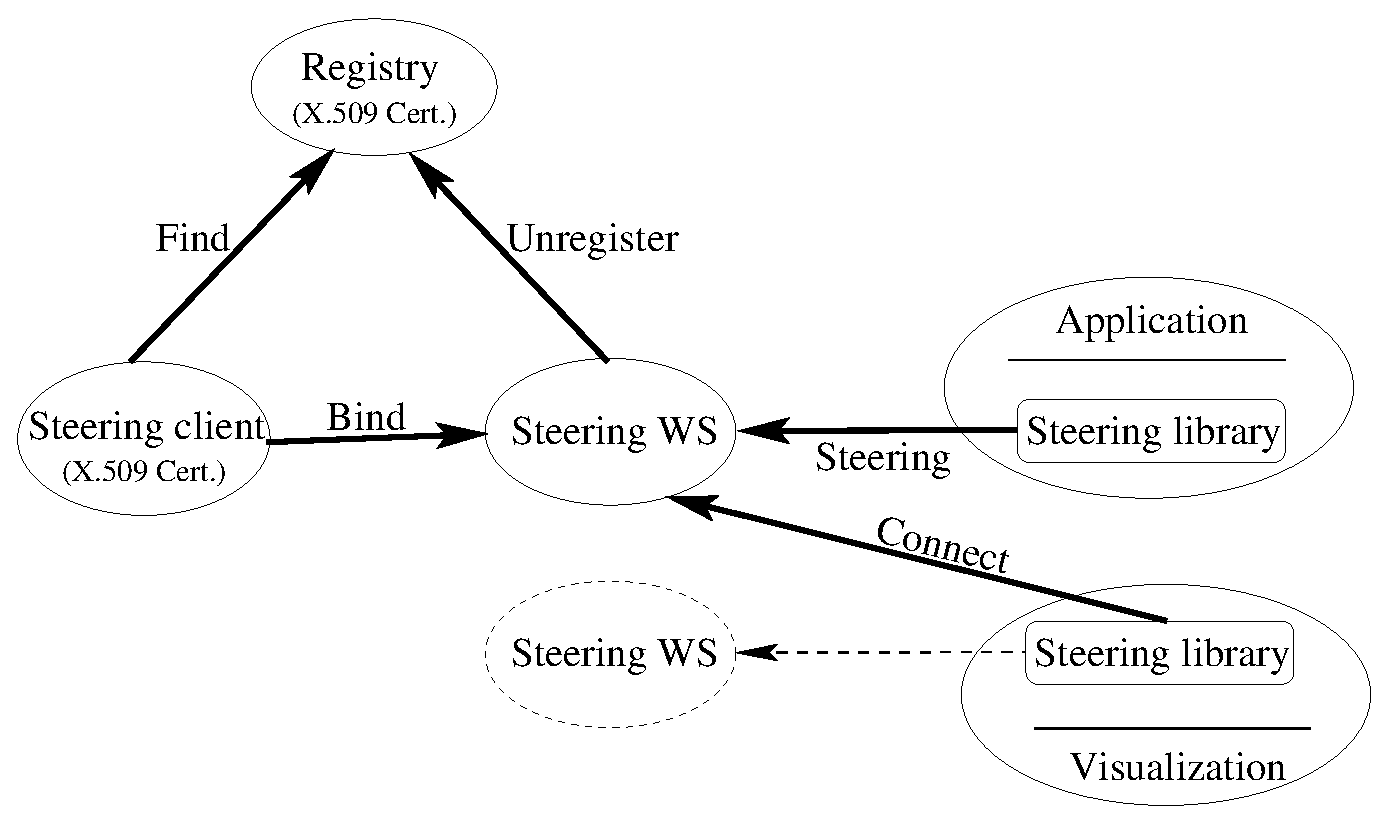
\includegraphics[width=14.0cm]{steer_ws_security.eps}
\end{center}
\caption{Illustration of the various connections that must be secured
within the RealityGrid framework.}
\label{fig:arch}
\end{figure}
Access to the registry, its entries and any actual SWS is controlled in
two ways; via SSL and e-Science X.509 certificates or via WS-Security
(WSSE) username and password.  The latter is essential in freeing us from
the requirement that a steerable application have access to an X.509 
certificate --- instead, it authenticates to the SWS using a passphrase
which is given to the SWS when it is created. In principle, each of
the remaining components in the architecture (shown in figure~\ref{fig:arch})
can have access to an
X.509 certificate and could therefore use mutually-authenticated SSL
which provides both authentication and encryption.

\begin{subsection}{The Registry}
The Registry may be secured using just WSSE or both WSSE and SSL.  For the
latter, it must be hosted in a secure WSRF::Lite container that has access to
a server X.509 certificate.  In our implementation, SSL takes priority over
WSSE so that a WSSE username/password is only checked for if no client
certificate is provided.  Every Registry must be given a passphrase when
it is created (using either \texttt{reg\_wsrf\_scripts/createReGFramework.pl}
or \texttt{reg\_wsrf\_scripts/createRegistry.pl}), irrespective of whether 
it will use SSL.  This allows those
services that do not have access to an X.509 certificate (such as the web-based
registry browser) to authenticate
themselves to the registry.
\end{subsection}

\begin{subsection}{Launching}
\label{sec:Launching}
The launching of a steerable job ({\it i.e.}\ one that has a SWS
associated with it) involves contacting a (WSRF::Lite) container,
creating the SWS and initializing it with a passphrase.  If the
container is secured using SSL (for which it requires access to a
server X.509 certificate), then the communication during this step is
encrypted and the passphrase for the SWS cannot be intercepted.
However, if the container is not secured then the passphrase for the
SWS will be transmitted in plain text at this stage.  If the client
authenticates to the Container using SSL then the Distinguished Name
(DN) of the client certificate is taken to be the identity of the root
user of the SWS.  If WSSE is used, then the supplied username is used
instead.

Once the SWS has been created, it must be registered.  This consists
of the client that created the SWS making a call to the \texttt{Add}
method of the Registry.  If the client authenticates to the Registry
using SSL then the DN of the client certificate is taken to be the
identity of the owner of that registry entry.  If WSSE is used, then
the supplied username is used instead.  An example of the Content
supplied when registering the SWS is shown in
figure~\ref{fig:contentXML}.  As can be seen, the
\texttt{componentContent} is augmented by a separate
\texttt{regSecurity} section which holds the passphrase of the SWS and
an array of users who have access to it.  The regServiceGroup code
uses this information to authenticate calls to get the {\bf Entry}
ResourceProperty while regServiceGroupEntry uses it to authenticate
calls that manage the registry entry itself ({\textit e.g.}\ attempts
to destroy it). Note that although \texttt{regSecurity} is a part of
the \texttt{Content} stored by the registry, the regServiceGroup
removes it before returning the \texttt{Content} to a user.

\begin{figure}
\begin{verbatim}
<Content>
  <registryEntry>
    <serviceType>SWS</serviceType>
    <componentContent>
      <componentStartDateTime>2006-03-13T12:46:38Z</componentStartDateTime>
      <componentCreatorName>/C=UK/O=eScience/OU=Manchester/L=MC/CN=andrew porter</componentCreatorName>
      <componentCreatorGroup>RSS Group</componentCreatorGroup>
      <componentSoftwarePackage>mini_app</componentSoftwarePackage>
      <componentTaskDescription>test wsrf work</componentTaskDescription>
    </componentContent>
    <regSecurity>
      <passphrase>somethingcunning</passphrase>
      <allowedUsers>
        <user>/C=UK/O=eScience/OU=Manchester/L=MC/CN=andrew porter</user>
      </allowedUsers>
    </regSecurity>
  </registryEntry>
</Content>
\end{verbatim}
\caption{Example of the Content supplied when registering a SWS.}
\label{fig:contentXML}
\end{figure}
When the program to be steered begins running, it must periodically contact the SWS.
Since it has no X.509 certificate it must authenticate to the SWS using WSSE.  The
steering library uses the username ``application'' and obtains the 
passphrase from the REG\_PASSPHRASE environment variable.
\end{subsection}


\begin{subsection}{On-line visualization}
On-line visualization (or any other configuration requiring that data
be sent from one component to another) is achieved by direct socket
connection between the simulation and visualization components.
Achieving such a connection requires that the visualization component
know where to connect to.  It retrieves this information from the SWS
associated with the simulation (indicated by the arrow labelled
``Connect'' in figure~\ref{fig:arch}).  Since it has no certificate,
it must use WSSE to authenticate to the simulation SWS and therefore
must have its passphrase.  This requirement is satisfied by ensuring
that the {\em same} passphrase is given to each of the SWSs representing
components that will be connected in some way.
\end{subsection} 

\begin{subsection}{Clean-up on job completion}
As indicated by the ``Unregister'' arrow in figure~\ref{fig:arch}, the SWS contacts
the Registry directly once the job has finished and the SWS is about to be destroyed.
Since the SWS has no X.509 certificate, authentication for this step is again via
WSSE.  The passphrase of the SWS is used to authenticate to the regServiceGroupEntry
service when calling its \texttt{Destroy} method.  As described in 
section~\ref{sec:Launching}, the
regServiceGroupEntry is able to check the passphrase since it is stored in the
\texttt{regSecurity} section of the {\bf Entry} ResourceProperty.
\end{subsection}

\end{section}

%---------------------------------------------------------------------

\begin{section}{The Registry service}
\label{sec:registry_service}

Once an SWS has been created, it may optionally be registered with a
Registry service.  The registry is implemented by a regServiceGroup
service and each entry in such a registry is implemented by a
regServiceGroupEntry service.  These services are based on the
WSRF::ServiceGroup and WSRF::ServiceGroupEntry services, respectively,
and have had certain methods overridden for the implementation of
security.

A service is registered via the \texttt{Add} method which, on
successful completion, returns a WS-Address containing information on
the regServiceGroupEntry that models the entry that has just been
created.  Calling \texttt{Destroy} on that regServiceGroupEntry
deletes the entry from the registry.

The services registered with a registry may be discovered by getting
the {\bf Entry} ResourceProperty of the registry using the standard
\texttt{GetResourceProperty} method:
\begin{verbatim}
$ans =  WSRF::Lite
        -> uri('http://www.ibm.com/xmlns/stdwip/web-services/WS-ResourceProperties')
        -> wsaddress(WSRF::WS_Address->new()->Address($target))
        -> GetResourceProperty(SOAP::Data->value(``Entry'')->type('xml') );
\end{verbatim}
Here, \$ans will be a SOAP::SOM object containing an array of Entry 
objects.

A web-based interface to the registry has been written and is available
from the RSS cvs repository ``ServiceGroupBrowser''.  This obviates the
need to install the various perl dependencies in order to be able to 
interact with the registry.

\end{section}

%---------------------------------------------------------------------

\begin{section}{Using the SWS for steering}
\label{sec:sws_steering}

In this section we will walk through the actions that must be taken in
order to steer an application via the SWS.

\begin{subsection}{Discovering the application}
When a client ({\it e.g.}\ a steering client) needs to know what
services are currently available, it must retrieve the {\bf Entry}
ResourceProperty from the Registry.  As described earlier, SSL or WSSE
can be used to authenticate this call.  The registry will only return
entries that the caller (as identified by their DN or username) is
authorised to see (as controlled by the \texttt{allowedUsers} array in
the \texttt{regSecurity} part of an entry's Content).
\end{subsection}

\begin{subsection}{Attaching to the application}
In order to be able to steer a job, a user must be able to
authenticate to the SWS.  If the SWS is hosted by a secure container
then the user can authenticate using SSL and will be granted access
provided their DN is in the list of the SWS' allowed users.  If SSL is
not available then the user may authenticate using WSSE which of
course requires that they know the passphrase of the SWS.

A user may be added to an SWS' list of allowed users by using the 
\texttt{SetResourceProperties} method to add their DN to the {\bf user}
ResourceProperty (see section~\ref{sec:swsMethods}).

Provided they can authenticate successfully, the client may either
call the \texttt{Attach} method (no arguments) of the SWS or use
\texttt{SetResourceProperties} to set the {\bf steererStatus} RP to
'ATTACHED'.  The \texttt{Attach} method returns an XML document describing the
commands that the application supports.  This document conforms to the
RealityGrid steering schema. Of course, these supported commands can
also be obtained by calling \texttt{GetResourceProperty} for the
{\bf supportedCommands} RP.

\end{subsection}

\begin{subsection}{Getting the parameter definitions}
Once a client has successfully attached to the SWS, the next stage is
to get the information published by the application.  The most
important aspect of this is the various monitored and steerable
parameters supported by the application.  This information is held on
the SWS in the {\bf paramDefinitions} ResourceProperty and therefore
can be accessed using some of the methods described in
section~\ref{sec:RPDoc}.  The information itself is an XML document
conforming to the RealityGrid steering schema.
\end{subsection}

\begin{subsection}{Getting the IOType and ChkType definitions}
As with the parameter definitions, the IOType and ChkType definitions
are also held as ResourceProperties ({\bf ioTypeDefinitions} and {\bf
chkTypeDefinitions}, respectively) on the SWS and therefore can be
accessed using the standard methods of section~\ref{sec:RPDoc}.
Again, the definitions are in the form of XML documents conforming to
the RealityGrid steering schema.  Note that all of these definitions
may be obtained in one go by getting the complete ResourceProperties
document of the service.  However, be aware that there may be a delay
between an application beginning execution and it actually setting
some of these ResourceProperties. Also, the Steering API permits a
program to change these definitions during execution.  It is therefore
essential to check for updates --- see section~\ref{sec:notification}.
\end{subsection}

\begin{subsection}{Getting status messages from the application}
Once a client has successfully obtained and parsed the parameter
definitions published by the application, it is ready to check for
status messages.  There are two ways of doing this.  The simplest is
to get the latest status message received by the SWS from the
application.  This is held in the {\bf latestStatusMsg} ResourceProperty and
is best obtained (especially on lightweight clients) by calling the
\texttt{GetResourceProperty} method.  The second, and more robust way of
obtaining status messages is to access the {\bf statusMsg} ResourceProperty.
This uses an array to buffer up to {\bf maxNumStatusMsg} (another
ResourceProperty) status messages.  Once the array is full, the
arrival of a new status message causes the oldest message held in the
buffer to be replaced.  Calling \texttt{GetResourceProperty} for this
ResourceProperty returns an XML document containing an array of status
messages in the form:
\begin{verbatim}
          <ResourceProperty>
            <statusMsg>
              <ReG_steer_message UID=`1'>
                <App_status>
                  ...
                </App_status>
              </ReG_steer_message>
              <ReG_steer_message UID=`2'>
                <App_status>
                  ...
                </App_status>
              </ReG_steer_message>
            </statusMsg>
          </ResourceProperty>
\end{verbatim}

As of version $2.0$ of the steering library, all steering messages are
given a unique identifer specified as an atrribute with name `Msg\_UID' on
the ReG\_steer\_message element.  This enables a client to check to see
whether it has seen the message before which is particularly useful
when getting the  {\bf latestStatusMsg} ResourceProperty.  This is because
this property is {\em only} changed when the application sends another
status message to the SWS --- it is unaffected by a client reading its
value.
\end{subsection}

\begin{subsection}{Sending control messages to the application}
In order to send a control message to the application a client must
construct a message conforming to the RealityGrid steering schema and
send it to the SWS by using the \texttt{SetResourceProperty} method to
set the {\bf controlMsg} ResourceProperty. {\it e.g.} To send a Stop
command the document that the client must supply as the argument to
the SetResourceProperty call would be:
\begin{verbatim}
          <wsrp:Insert>
            <controlMsg>
              <ReG_steer_message>
                <Steer_control>
                  <Command>
                    <Cmd_name>STOP</Cmd_name>
                  </Command>
                </Steer_control>
              </ReG_steer_message>
            </controlMsg>
          </wsrp:Insert>
\end{verbatim}
\end{subsection}

\begin{subsection}{Checking for `notifications'}
\label{sec:notification}
It is important that a client check for notifications from the steered
application in order that it can take action when, for example, the
set of parameters registered by the application changes.  Support for
this feature is included in the SWS through the {\bf lastModifiedTime}
ResourceProperty which records the last time (in the form of a single
integer holding the number of seconds since the UNIX epoch) that the
ResourceProperty Document was modified.  It is important to note that
this parameter is {\em not} changed by the setting of either the {\bf
statusMsg} or {\bf controlMsg} ResourceProperties since the frequency
with which those two properties are likely to be set would limit its
usefulness.

In contrast to the SGS, the SWS does not explicitly notify any
attached steering clients that the application has finished running.
Instead, once the application has finished ({\it i.e.} has called
Steering\_finalize or caught a signal) the SWS unregisters itself from
the registry and then expires.  Thus, any attached steering client is
effectively notified of the application's completion by the
disappearance of the SWS.
\end{subsection}

\begin{subsection}{Detaching from the application}
The steering client notifies the SWS that it has finished steering the
application either by calling the \texttt{Detach} method or by calling
\texttt{SetResourceProperty} for {\bf steererStatus} with a value of
'DETACHED'.  Unlike the SGS, the SWS does not explicitly acknowledge
a call to \texttt{Detach}.  (However, the value of the {\bf clientCount}
ResourceProperty will be decremented by one upon a successful detach.)
If there are no steering clients attached to the SWS then the
application ceases to emit status messages to it.
\end{subsection}

\end{section}

%---------------------------------------------------------------------

\begin{section}{The Methods of the SWS}
\label{sec:swsMethods}

Table~\ref{table:SWSmethods} lists all of the methods supported by the
SWS.

\begin{table}
\begin{center}
\begin{tabular}{l|p{4cm}|p{4cm}|p{3cm}}
\hline\hline
Method & Description & Arguments & Returns\\
\hline
AddChild & Adds a child service to the SWS 
& EPR of child service  
& Fault on failure \\

Attach & Attach to the application & -- 
& XML doc containing supported commands\\

GetParamLog & Called by a steering client to retrieve logged parameter values 
& Handle of parameter 
& Space-delimited list of values (cast as doubles), string \\

PutParamLog & Called by the application to save logged parameter values 
& Logged parameter values as a space-delimited list in CDATA block
& Fault on failure \\

RecordCheckpoint & Called by the application to register a checkpoint 
& XML listing files (string) and XML meta-data (string)
& Fault on failure \\

Detach & Detach from the application & -- & --\\
\hline
Destroy & Destroy the SWS and remove any associated registry entry & -- &--\\
GetResourceProperty & Get a single RP & Name of the RP (string) 
& Value of the RP \\

GetResourcePropertyDocument & Get the whole ResourceProperty doc 
& -- & The RP doc\\

GetMultipleResourceProperties & Get one or more RPs 
& Names of the RPs in XML doc & Value(s) of the RP(s) \\
SetResourceProperties & Set the value of one or more RPs 
& XML with new RP values tagged with RP names & -- \\
\hline\hline
\end{tabular}
\end{center}
\caption{The methods of the SWS.  Those in the lower section of the table 
are standard WS-RF methods (only the most useful of these are listed).}
\label{table:SWSmethods}
\end{table}

\end{section}

\end{document}
